\documentclass[printmode]{mgr}

\usepackage[polish]{babel}
\usepackage[utf8]{inputenc}
\usepackage{fontenc}
\usepackage{polski}
\usepackage{graphicx}
\usepackage{subfigure}
\usepackage{psfrag}
\usepackage{supertabular}
\usepackage{array}
\usepackage{hhline}
\usepackage{indentfirst}
\usepackage{float}
\usepackage{enumitem}
\usepackage{afterpage}
\usepackage{tabularx}
\usepackage{listings}
\usepackage{color, colortbl}
\usepackage{hyphenat}
\usepackage[hidelinks]{hyperref}
\usepackage{ucs}
\usepackage{makecell}
\usepackage[edges]{forest}
\usepackage{tikz}
\usepackage{pgfplots}
\usepackage{pgfplotstable}

\def\Size{4pt}
\tikzset{%
  folder/.pic={%
    \filldraw [draw=folderborder, top color=folderbg!50, bottom color=folderbg] (-1.05*\Size,0.2\Size+5pt) rectangle ++(.75*\Size,-0.2\Size-5pt);
    \filldraw [draw=folderborder, top color=folderbg!50, bottom color=folderbg] (-1.15*\Size,-\Size) rectangle (1.15*\Size,\Size);
  },
  file/.pic={%
    \filldraw [draw=folderborder, top color=folderbg!5, bottom color=folderbg!10] (-\Size,.4*\Size+5pt) coordinate (a) |- (\Size,-1.2*\Size) coordinate (b) -- ++(0,1.6*\Size) coordinate (c) -- ++(-5pt,5pt) coordinate (d) -- cycle (d) |- (c) ;
  },
}

\forestset{%
  declare autowrapped toks={pic me}{},
  pic dir tree/.style={%
    for tree={%
      folder,
      font=\ttfamily,
      grow'=0,
    },
    before typesetting nodes={%
      for tree={%
        edge label+/.option={pic me},
      },
    },
  },
  pic me set/.code n args=2{%
    \forestset{%
      #1/.style={%
        inner xsep=2\Size,
        pic me={pic {#2}},
      }
    }
  },
  pic me set={directory}{folder},
  pic me set={file}{file},
}

\makeatletter
\pgfplotsset{
    /pgfplots/flexible xticklabels from table/.code n args={3}{%
        \pgfplotstableread[#3]{#1}\coordinate@table
        \pgfplotstablegetcolumnbyindex{#2}\of{\coordinate@table}\to\pgfplots@xticklabels
        \let\pgfplots@xticklabel=\pgfplots@user@ticklabel@list@x
    }
}
\makeatother
\raggedbottom

\definecolor{mygreen}{rgb}{0,0.6,0}
\definecolor{mygray}{rgb}{0.5,0.5,0.5}
\definecolor{mymauve}{rgb}{0.58,0,0.82}
\definecolor{lightgray}{rgb}{.9,.9,.9}
\definecolor{darkgray}{rgb}{.4,.4,.4}
\definecolor{purple}{rgb}{0.65, 0.12, 0.82}
\definecolor{folderbg}{RGB}{124,166,198}
\definecolor{folderborder}{RGB}{110,144,169}

\lstdefinelanguage{JavaScript}{
  keywords={break, case, catch, continue, debugger, default, delete, do, else, false, finally, for, function, if, in, instanceof, new, null, return, switch, this, throw, true, try, typeof, var, void, while, with, \$scope},
  morecomment=[l]{//},
  morecomment=[s]{/*}{*/},
  morestring=[b]',
  morestring=[b]",
  ndkeywords={class, export, boolean, throw, implements, import, this},
  keywordstyle=\color{blue}\bfseries,
  ndkeywordstyle=\color{darkgray}\bfseries,
  identifierstyle=\color{black},
  commentstyle=\color{purple}\ttfamily,
  stringstyle=\color{mymauve}\ttfamily,
  sensitive=true
}

\lstdefinelanguage{Slim}{
  keywords={ul, div, a, href, i, li},
  morecomment=[l]{//},
  morecomment=[s]{/*}{*/},
  morestring=[b]',
  morestring=[b]",
  ndkeywords={class, export, boolean, throw, implements, import, this},
  keywordstyle=\color{blue}\bfseries,
  ndkeywordstyle=\color{darkgray}\bfseries,
  identifierstyle=\color{black},
  commentstyle=\color{purple}\ttfamily,
  stringstyle=\color{mymauve}\ttfamily,
  sensitive=true,
}

\lstset{ %
  backgroundcolor=\color{white},   % choose the background color
  basicstyle=\footnotesize,        % size of fonts used for the code
  breaklines=true,                 % automatic line breaking only at whitespace
  frame=single,  
  commentstyle=\color{mygreen},    % comment style
  escapeinside={\%*}{*)},          % if you want to add LaTeX within your code
  keywordstyle=\color{blue},       % keyword style
  stringstyle=\color{mymauve},     % string literal style
  tabsize=2,
  inputencoding=utf8x, 
  extendedchars=\true,
  literate={ą}{{\k{a}}}1
  {Ą}{{\k{A}}}1
  {ę}{{\k{e}}}1
  {Ę}{{\k{E}}}1
  {ó}{{\'o}}1
  {Ó}{{\'O}}1
  {ś}{{\'s}}1
  {Ś}{{\'S}}1
  {ł}{{\l{}}}1
  {Ł}{{\L{}}}1
  {ż}{{\.z}}1
  {Ż}{{\.Z}}1
  {ź}{{\'z}}1
  {Ź}{{\'Z}}1
  {ć}{{\'c}}1
  {Ć}{{\'C}}1
  {ń}{{\'n}}1
  {Ń}{{\'N}}1
}

\newcommand\blankpage{%
  \null
  \thispagestyle{empty}%
  \addtocounter{page}{-1}%
  \newpage}

\addto\extraspolish{\def\bibname{Literatura}\let\refname\bibname}
\renewcommand{\lstlistingname}{Fragment kodu}

\date{2017}

\title{Analiza porównawcza frameworków internetowych w~języku Ruby w~zastosowaniach GISowych}
\engtitle{Comparative analysis of Ruby's web frameworks for Geographic Information Systems}
\author{Mikołaj Grygiel}
\supervisor{dr inż. Roman Ptak, W4/K9}

\field{Informatyka (INF)}
\specialisation{ Inżynieria systemów informatycznych (INS)}

\begin{document}
\bibliographystyle{plabbrv}

\maketitle

\tableofcontents




\chapter{Badania}

\section{Plan badań}

Na podstawie dostępnej dokumentacji oraz zaimplementowanych aplikacji w~każdym z~badanych narzędzi, frameworki zostaną porównane w~następujących aspektach:
\begin{itemize}
  \item dostępne funkcjonalności
  \item struktura utworzonego projektu
  \item wydajność zaimplementowanej aplikacji
\end{itemize}


\subsection{Aplikacja zaimplementowana na potrzeby badań}

W~celu wykonania analizy porównawczej w~każdym z~wybranych frameworków została zaimplementowana aplikacja internetowa operująca na danych geograficznych posiadająca takie same funkcjonalności. Aplikacje zostały zrealizowane zgodnie z~architekturą i~konwencją wykorzystywaną w~danym frameworku zawartych w~dokumentacji narzędzia. W projektach wykorzystano jedynie biblioteki niezbędne do zrealizowania wymaganych funkcjonalności. Nie używano bibliotek modyfikujących architekturę aplikacji lub funkcjonalności frameworka.
Aplikacja ma za zadanie wykonywać 4 podstawowe operacje na danych geograficznych:
\begin{itemize}
  \item tworzenie
  \item odczytywanie
  \item aktualizowanie
  \item usuwanie
\end{itemize}

Wszystkie funkcjonalności wykonanej aplikacji zostały zaprezentowane na rysunku \ref{fig:use_cases}.

\begin{figure}[H]
  \centering
  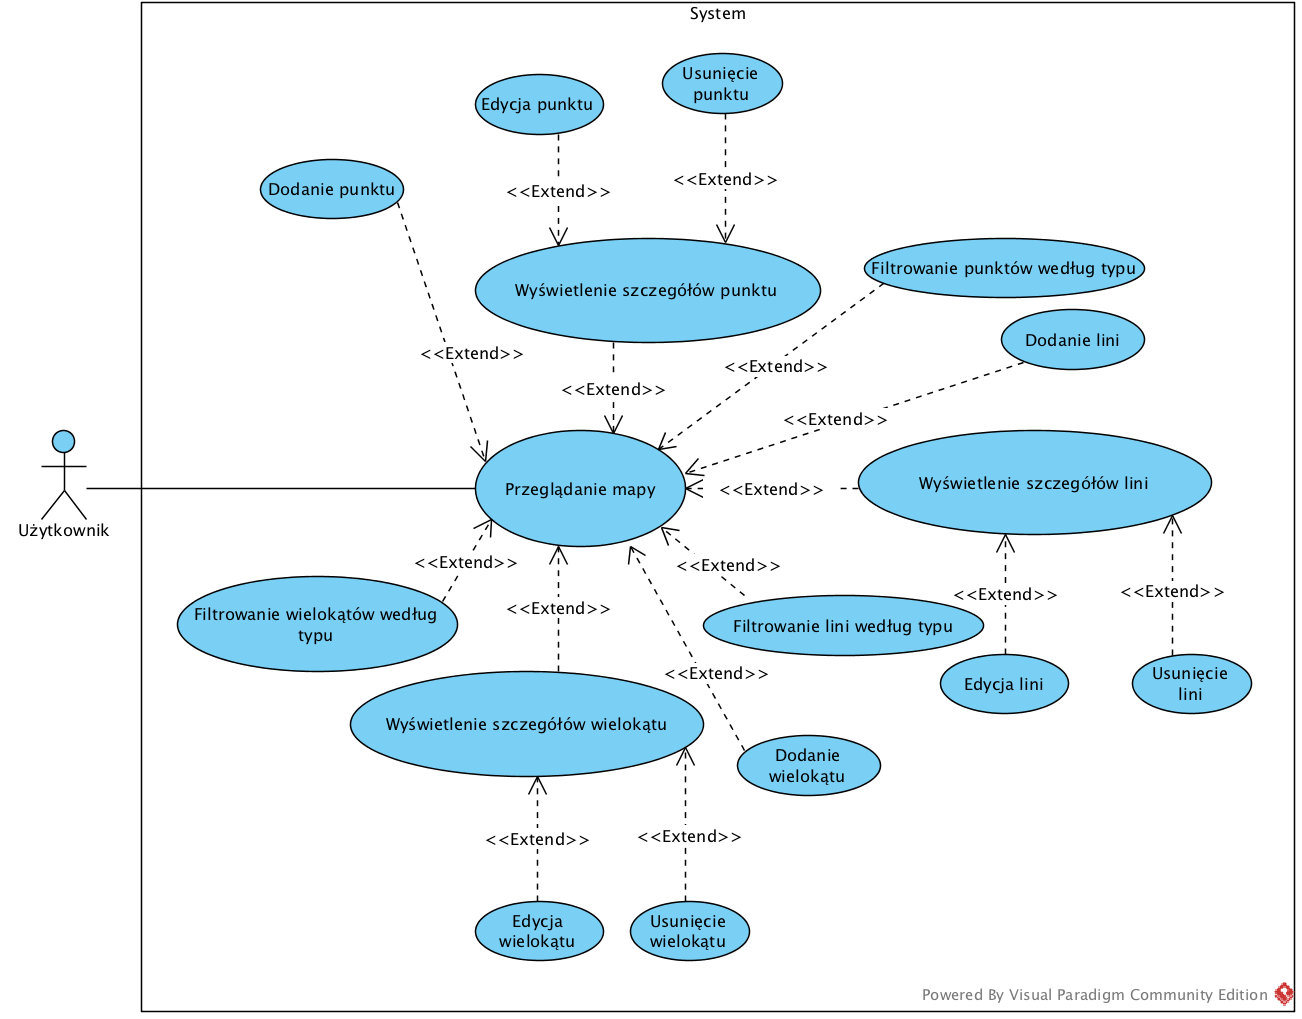
\includegraphics[width=1\linewidth]{pictures/use_cases}
  \caption{Diagram przypadków użycia aplikacji}
  \label{fig:use_cases}
\end{figure}

Aby przeprowadzić badania w~realistycznych warunkach aplikacja korzysta z~gotowych zbiorów danych:
\begin{itemize}
  \item Punkty - pochodzące ze zbioru "Państwowy rejestr nazw geograficznych - miejscowości", zbiór zawiera 256796 obiektów, dostępny jest pod adresem http://www.codgik.gov.pl/index.php/darmowe-dane/prng.html.
  \item Linie - dane uzyskano z~serwisu http://download.geofabrik.de/europe/poland.html pozwalającego pobrać drogi z~terenu Polski z~bazy danych OpenStreetMap. Zbiór obejmuje 2519660 obiektów.
  \item Wielokąty - obiekty pobrano z~Państwowego Rejestru Granic dostępnego pod adresem http://gis-support.pl/baza-wiedzy/dane-do-pobrania/, zbiór liczy 59978 obiektów.
\end{itemize}

Każda wersja aplikacji posiada taką samą bazę danych, której schemat znajduje się na rysunku \ref{fig:erd}. Jako bazę danych wykorzystano PostgreSQL z~rozszerzeniem PostGIS. Dane geograficznej w~warstwie aplikacji przetwarzano używając biblioteki RGeo.

\begin{figure}[H]
  \centering
  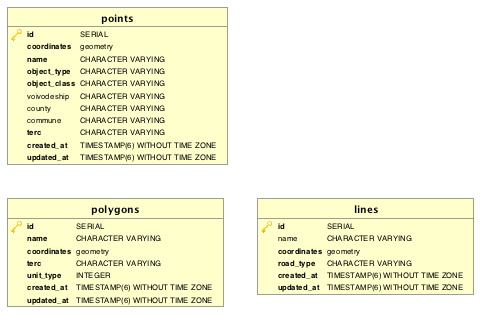
\includegraphics[width=1\linewidth]{pictures/erd}
  \caption{Schemat ERD bazy danych}
  \label{fig:erd}
\end{figure}

Do prezentacji danych na mapie wykorzystano bibliotekę LefletJS, ponieważ jest darmowa i~ma otwarte źródła. Mapa pochodzi z~serwisu OpenStreetMap. Widok gotowej aplikacji znajduje się na rysunku \ref{fig:app}.

\begin{figure}[H]
  \centering
  \includegraphics[width=1\linewidth]{pictures/app}
  \caption{Widok gotowej aplikacji}
  \label{fig:app}
\end{figure}

\subsection{Narzędzia wykorzystane podczas badań}
Do zmierzenia wydajności zaimplementowanych aplikacji zastosowano następujące narzędzia:
\begin{itemize}
  \item{Capybara} - biblioteka w~języku Ruby pozwalająca symulować interakcje prawdziwego użytkownika z~wybraną aplikacją internetową. Capybara dostarcza szereg metod pozwalających zapisać jako scenariusz kolejne kroki postępowania użytkownika m.in. kliknięcie wybranego elementu lub wprowadzenie danych do formularza. Do wspierania JavaScriptu, Capybara używa Selenium. Selenium jest narzędziem, które umożliwia automatyczne wykonanie testów akceptacyjnych aplikacji internetowej w~wybranej przeglądarce. W przeprowadzonych badaniach testy uruchomione zostały w~przeglądarce Firefox. \cite{doc_capybara}
  \item{JMeter} - aplikacja napisana w~języku Java dostępna na licencji otwartego źródła. JMeter służy do wykonywania testów wydajności aplikacji internetowych. W niniejszych badaniach JMeter wykorzystywał protokół HTTP do wysyłania określonych zapytań do aplikacji. W badaniach pomocna również okazała się funkcja symulowania wielu użytkowników - JMeter uruchamia wybrany scenariusz na wielu wątkach aby sprawdzić jak zachowa się aplikacja przy wielu równoległych zapytaniach. \cite{doc_jmeter}
  \item{Ruby Benchmark} - biblioteka pozwalająca na zmierzenie czasu wykonywania podanego blogu kodu. Ruby Benchmark został wykorzystany przy zmierzeniu czasu wykonywania scenariuszy utworzonych przy pomocy Capybary oraz czasu wykonywania operacji na bazie danych. \cite{doc_benchmark}
\end{itemize}

\subsection{Środowisko badawcze}

Do przeprowadznia badań użyto dwóch komputerów:

\begin{enumerate}
\item Komputer - serwer
  \begin{itemize}
    \item MacBook Pro(Retina, 13 cali,model: Early 2015)
    \item Procesor: Intel Core i5 2,7 GHz 2 rdzenie
    \item Pamięć RAM: 8GB DDR3 1867 MHz
    \item Dysk: 120GB APPLE SSD SM0128G
  \end{itemize}
\item Komputer - tester
  \begin{itemize}
    \item MacBook Mini 6.1
    \item Procesor: Intel Core i5 2,5 GHz 2 rdzenie
    \item Pamięć RAM: 8GB DDR3 1600 MHz
    \item Dysk: 240GB GOODRAM SSD CX100
  \end{itemize}
\end{enumerate}

Na \textit{komputerze - serwer} uruchomiona była aktualnie testowana aplikacja. \textit{Komputer - tester} wykonywał zaimplementowane badania. Podczas badań komputery były podłączone ze sobą lokalnie przy pomocy sieci Wi-Fi 802.11n i~nie miały dostępu do zewnętrznej sieci. Na komputerach uruchomione były tylko niezbędne aplikacje do przeprowadzenia badań.

\section{Porównanie funkcjonalności wybranych frameworków}

\subsection{Przechowywanie danych}

 Ruby on Rails posiada największe wsparcie w~przechowywaniu danych geograficznych z~rozpatrywanych narzędzi. Biblioteka ActiveRecord domyślne wykorzystywana w~Ruby on Rails do mapowania obiektowo-relacyjnego posiada adaptery dla następujących baz danych: PostgreSQL z~dodatkiem PostGIS, MysqlSpatial, SpatiaLite. Za pomocą adapterów, w~migracjach można używać typów kolumn z~przestrzennych baz danych. Przy komunikacji typy przestrzenne z~bazy danych mapowane są na typy zaimplementowane w~bibliotece RGeo. Konfiguracja nie wymaga wiele pracy, wystarczy dodać odpowiednią bibliotekę do projektu i~w konfiguracji bazy danych ustawić odpowiedni adapter. Od tego momentu można w~migracjach przy definiowaniu kolumn używać wszystkich typów przestrzennych dostarczanych przez wybraną bazę danych. Dane przestrzenne podczas wykonywanych akcji między aplikacją, a~bazą danych są automatycznie mapowane.

 Tworzenie bazy danych przestrzennej za pomocą Rody nie stanowi problemu. Framework pozwala używać kodu SQL w~migracjach dlatego można włączyć dowolne rozszerzenie wybranej bazy danych i~używać dodatkowych typów. Roda nie zapewnia specjalnego wsparcia przy mapowaniu danych przestrzennych na obiekty, dane są zwracane w~formie tekstowej binarnej wartości pola.

 Hanami w~migracjach pozwala ozywać kodu napisanego w~języku SQL do np. definiowania typów lub włączania dodatków w~bazie danych, dlatego bez problemów można stworzyć i~wersjonować bazę danych z~typami przestrzennymi. Jednak framework, podobnie jak Ruby on Rails, posiada mechanizm automatycznego mapowania typów bazy danych do typów obiektów, który nie pozwala na definiowanie własnych typów lub własnych reguł mapowania. To ograniczenie powoduje otrzymanie wyjątku przy próbie uruchomienia aplikacji zawierającej nieznany typ. Framework wspiera jedynie typy przestrzenne zdefiniowane w~bazie danych PostgreSQL, które są zapisywane postaci tekstowej zawierającej współrzędne. Możliwe jest zapisanie wszystkich 3 podstawowych typów przestrzennych: punktu, linii, wielokąta. PostgreSQL dostarcza podstawowe operacje wyszukiwania danych przestrzennych tylko dla punktów, dlatego zastosowanie PostgreSQL bez dodatku PostGIS mocno ogranicza możliwości budowanej aplikacji. Dodanie obsługi typów geometrycznych dostarczonych przez dodatek PostGIS nie wymaga dużej ilości kodu, wymagana jest dobra znajomość języka Ruby i~mechanizmu przedefiniowania istniejących już klas tzw. "monkey patching". Najłatwiejsze rozwiązanie pozwalające używać typów geometrycznych z~biblioteki PostGIS znajduje się na listingu \ref{lst:postgis_patching}. Przy takim rozwiązaniu wartości z~kolumny geometrycznej mapowane są na typ String z~wartością binarną.

 \newpage

\begin{lstlisting}[language=Ruby, caption={Obsługa typów geometrycznych z~biblioteki PostGIS przez Hanami}, label=lst:postgis_patching]
require 'rom/sql/extensions/postgres/inferrer'
require 'rom/sql/extensions/postgres/types'

ROM::SQL::Schema::PostgresInferrer.class_eval do
  alias map_db_type_original map_db_type

  def map_db_type(db_type)
    # najpierw następuje próba użycia oryginalnej metody mapowania typów
    # jeśli zakończy się ona nie powodzeniem, to następuje sprawdzenie 
    # czy typ kolumny z~bazy danych rozpoczyna się od słowa 'geometry'
    # wtedy dane są rzutowane do typu ROM::Types::String
    map_db_type_original(db_type) || (db_type.start_with?('geometry') ? ROM::Types::String : nil)
  end
end
\end{lstlisting}

\subsection{Obiektowe przetwarzanie danych}

 Do obiektowego przetwarzania danych dostępne są dwie biblioteki Rgeo i~GeoRuby. Ruby on Rails, dzięki wspomnianym wcześniej adapterom dużo wygodniej jest korzystać z~Rgeo dzięki automatycznemu mapowaniu danych relacyjnych na obiekty.
 Frameworki Roda oraz Hanami w~żaden sposób nie rozszerzają możliwości bibliotek Rgeo i~GeoRuby. W  Hanami, zaimplementowana metoda mapująca wartości przestrzenne na typ obiektowy zwraca wartość binarną, Roda domyślne zwraca dane przestrzenne w~takiej formie. Wartość binarną dalej można zamienić na typ z~biblioteki Rgeo, co zaprezentowano na listingu \ref{lst:coordinates_helper}

 \begin{lstlisting}[language=Ruby, caption={Tworzenie obiektu Rgeo z~zapisu binarnego danych przestrzennych}, label=lst:coordinates_helper]
module CoordinatesHelper
  FACTORY = RGeo::Geographic.spherical_factory(:srid => 4326)

  # utworzenie obiektu Rgeo z~binarnego zapisu danych przestrzennych
  def coordinates_object
    RGeo::WKRep::WKBParser.new(FACTORY, support_ewkb: true,
        default_srid: 4326).parse(coordinates)
  end

  # rzutowanie obiektu przestrzennego do postaci "well known text"
  def coordinates_text
    coordinates_object.as_text
  end
end
\end{lstlisting}

\subsection{Prezentowanie danych}

Framework Ruby on Rails posiada biblioteki do integracji obu narzędzi do prezentacji danych geograficznych wspomnianych w~rozdziale \ref{sec:maps-tools}:
\begin{enumerate}
  \item{leaflet-rails} - dołącza do projektu Ruby on Rails bibliotekę leafletjs napisaną w~języku JavaScript wraz ze stylami oraz dodaje metody do widoków pozwalające na dołączenie mapy i~podstawową konfiguracje bez potrzeby używania JavaScriptu.
  \item{Google Maps for Rails} - biblioteka opakowuje JavaScriptową bibliotekę GoogleMaps JavaScript API, ułatwiając jej dodanie do projektu.
\end{enumerate}
Dzięki takiej integracji zgodnie z~sposobem dołączania bibliotek do projektu w~języku Ruby \cite{doc_ruby}, wspomniane biblioteki są przechowywane centralnie w~systemie zamiast w~projekcie.
Roda oraz Hanami w~przeciwieństwie do Ruby on Rails nie posiadają bibliotek wspomagających dołączenie do projektu biblioteki Leafletjs lub Google Maps Javascript API. Żeby skorzystać jednej z~wymienionych bibliotek należy dołączyć jej kod do projektu.

Przy odczycie danych w~formacie JSON, Ruby on Rails oraz Roda automatycznie serializują model do postaci JSON. W projekcie wykorzystującym Hanami, niezbędne jest dodanie zewnętrznej bilbioteki realizującej serializowanie danych np. \textit{Roar} i~zdefiniowanie odpowiedniego prezentera. Przykładowy prezenter został zaprezentowany na listingu \ref{lst:representer}

 \begin{lstlisting}[language=Ruby, caption={Prezenter dla modelu Point}, label=lst:representer]
require 'roar/decorator'
require 'roar/json'

module Web::Representers
  class Point < Roar::Decorator
    include Roar::JSON

    property :id
    property :name
    property :object_type
    property :object_class
    property :voivodeship
    property :county
    property :commune
    property :terc
    property :coordinates_text
    property :color
  end
end
\end{lstlisting}

\subsection{Podsumowanie}

Ruby on Rails posiada zdecydowanie najwięcej gotowych narzędzi do pracy z~danymi geograficznymi z~rozpatrywanych frameworków. Tworzenie aplikacji dzięki temu trwa mniej czasu. Roda mimo mniejszego wsparcia dla danych przestrzennych w~przeciwieństwie do Hanami pozwala na ich używanie bez rozszerzania funkcjonalności frameworka. Hanami pozwala zbudować prosty system GIS wykorzystujący podstawowe typy przestrzenne dostępne w~bazie danych PostgreSQL, ale implementacja systemu informacji geograficznej wykorzystującego inną bazę danych za pomocą frameworku Hanami wymaga od programisty znacznie więcej pracy i~większych umiejętności programistycznych aby rozszerzyć możliwości frameworka.

\newpage

\section{Porównianie struktur wykonanych projektów}

Struktura zaimplementowanego projektu przy pomocy Ruby on Rails bezpośrednio odzwierciedla architekturę frameworku. W projekcie mamy jasny podział na Model-Widok-Kontroler. 

\begin{figure}[H]
  \centering
  \begin{minipage}[H]{0.4\textwidth}
    \begin{forest}
      pic dir tree,
      where level=0{}{% folder icons by default; override using file for file icons
        directory,
      },
      [rails\_project
        [app
          [assets
            [javascripts
              [application.js 17, file]
              [checkboxes.js 72, file]
              [line\_form.js 33, file]
              [lines.js 38, file]
              [point\_form.js 33, file]
              [points.js 65, file]
              [polygon\_form.js 33, file]
              [polygons.js 36, file]
              [map.js 41, file]
            ]
            [stylesheets
              [application.scss 54, file]
            ]
          ]
          [controllers
            [application\_controller.rb 3, file]
            [lines\_controller.rb 50, file]
            [maps\_controller.rb 7, file]
            [points\_controller.rb 56, file]
            [polygons\_controller.rb 50, file]
          ]
        ]
      [...]]
    \end{forest}
  \end{minipage}
  \hfill
  \begin{minipage}[t!]{0.4\textwidth}
    \begin{forest}
      pic dir tree,
      where level=0{}{% folder icons by default; override using file for file icons
        directory,
      },
      [...
        [models
          [concerns
            [gis\_support.rb 15, file]
          ]
          [application\_record.rb 3, file]
          [line.rb 23, file]
          [point.rb 32, file]
          [polygon.rb 18, file]
        ]
        [views
          [layouts
            [application.html.erb 12, file]
          ]
          [maps
            [index.html.erb 91, file]
          ]
          [shared
            [\_line\_form.erb 11, file]
            [\_point\_form.html.erb 16, file]
            [\_polygon\_form.html.erb 13, file]
          ]
        ]
      ]
    \end{forest}
  \end{minipage}
  
    
  \caption{Struktura projektu Ruby on Rails}
  \label{fig:rails_proj_structure}
\end{figure}

\newpage
Filozofia prostoty w~frameworku Roda ma swoje odzwierciedlenie w~strukturze projektu, która nie posiada za wiele rozgałęzień.

\begin{figure}[H]
  \centering
  \begin{minipage}[H]{0.4\textwidth}
    \begin{forest}
      pic dir tree,
      where level=0{}{% folder icons by default; override using file for file icons
        directory,
      },
      [roda\_project
        [assets
          [js
            [application.js 17, file]
            [checkboxes.js 63, file]
            [leaflet.js 5, file]
            [line\_form.js 58, file]
            [lines.js 39, file]
            [point\_form.js 59, file]
            [points.js 66, file]
            [polygon\_form.js 60, file]
            [polygons.js 37, file]
            [map.js 41, file]
          ]
          [css
            [leaflet.css 548, file]
            [main.css.scss 34, file]
          ]
        ]
      [...]]
    \end{forest}
  \end{minipage}
  \hfill
  \begin{minipage}[t!]{0.4\textwidth}
    \begin{forest}
      pic dir tree,
      where level=0{}{% folder icons by default; override using file for file icons
        directory,
      },
      [...
        [models
          [concerns
            [gis\_support.rb 16, file]
          ]
          [line.rb 20, file]
          [point.rb 23, file]
          [polygon.rb 19, file]
        ]
        [routes
          [lines.rb 47, file]
          [points.rb 47, file]
          [polygons.rb 47, file]
        ]
        [views
          [shared
            [\_line\_form.erb 12, file]
            [\_point\_form.erb 17, file]
          ]
          [index.erb 92, file]
          [layout.erb 14, file]
        ]
        [app.rb 33, file]
        [models.rb 24, file]
      ]
    \end{forest}
  \end{minipage}  
  \caption{Struktura projektu Roda}
  \label{fig:roda_proj_structure}
\end{figure}

Dodatkowe warstwy abstrakcji w~architekturze projektu Hanami przekładają się na bardziej rozbudowaną strukturę projektu.

\begin{figure}[H]
  \centering
  \begin{minipage}[H]{0.4\textwidth}
    \begin{forest}
      pic dir tree,
      where level=0{}{% folder icons by default; override using file for file icons
        directory,
      },
      [hanami\_project
        [apps
          [web
            [assets
              [javascripts
                [application.js 17, file]
                [checkboxes.js 63, file]
                [leaflet.js 5, file]
                [line\_form.js 58, file]
                [lines.js 39, file]
                [point\_form.js 59, file]
                [points.js 66, file]
                [polygon\_form.js 60, file]
                [polygons.js 37, file]
                [map.js 41, file]
              ]
              [stylesheets
                [leaflet.css 548, file]
                [main.css.scss 34, file]
              ]
            ]
            [templates
              [map
                [index.html.erb 86, file]
              ]
              [shared
                [\_line\_form.html.erb 22, file]
                [\_point\_form.html.erb 42, file]
                [\_polygon\_form.html.erb 26, file]
              ]
              [application.html.erb 30, file]
            ]
          ]
        ]
      [...]]
    \end{forest}
  \end{minipage}
  \hfill
  \begin{minipage}[t!]{0.4\textwidth}
    \begin{forest}
      pic dir tree,
      where level=0{}{% folder icons by default; override using file for file icons
        directory,
      },
      [...
        [controllers
          [lines
            [create.rb 31, file]
            [destroy.rb 9, file]
            [index.rb 23, file]
            [update.rb 30, file]
          ]
          [points
            [create.rb 37, file]
            [destroy.rb 9, file]
            [index.rb 24, file]
            [update.rb 36, file]
          ]
          [polygons
            [create.rb 32, file]
            [destroy.rb 9, file]
            [index.rb 23, file]
            [update.rb 32, file]
          ]
          [map
            [index.rb 7, file]
          ]
        ]
        [representers
          [line.rb 12, file]
          [point.rb 17, file]
          [polygon.rb 13, file]
        ]
        [views
          [map
            [index.rb 26, file]
          ]
          [application\_layout.rb 7, file]
        ]
        [application.rb 65, file]
      ]
    \end{forest}
  \end{minipage}
  
    
  \caption{Struktura projektu Hanami - część I}
  \label{fig:hanami_1_proj_structure}
\end{figure}

\begin{figure}[H]
  \centering
  \begin{forest}
    pic dir tree,
    where level=0{}{% folder icons by default; override using file for file icons
      directory,
    },
    [hanami\_project
      [lib
        [web
          [entities
            [line.rb 16, file]
            [point.rb 19, file]
            [polygon.rb 15, file]
          ]
          [repositories
            [concerns
              [coordinates\_helper.rb 10, file]
              [gis\_support.rb 16, file]
            ]
            [line\_repository.rb 7, file]
            [point\_repository.rb 7, file]
            [polygon\_repository.rb 7, file]
          ]
        ]
        [postgres\_inferrer.rb 8, file]
      ]
    ]
  \end{forest}   
  \caption{Struktura projektu Hanami - część II}
  \label{fig:hanami_2_proj_structure}
\end{figure}

Na rysunkach \ref{fig:files_count} i~\ref{fig:folders_count} można zauważyć, że projekt stworzony przy pomocy Hanami zawiera znacznie więcej plików i~folderów od dwóch pozostałych projektów. Dodatkowe warstwy abstrakcji w~architekturze frameworka przekładają się na bardziej skomplikowaną strukturę projektu. Projekty zrealizowany przy pomocy Ruby on Rails i~Roda zawierają dokładnie tyle samo plików, ale Roda ma nieco mniej folderów. Na rysunku \ref{fig:roda_proj_structure} można zauważyć, że struktura projektu Roda jest bardziej płaska niż struktura Ruby on Rails zaprezentowana na rysunku \ref{fig:rails_proj_structure}.

\begin{figure}[H]
  \centering
  \begin{tikzpicture}
    \begin{axis}[
      width = 0.8\linewidth,
      height = 0.5\linewidth,
      ybar=50pt,
      enlarge x limits=0.15,
      ymin=0,
      xtick=\empty,
      legend cell align=left, legend pos=outer north east,
      ylabel={Liczba plików},
      nodes near coords,
      nodes near coords align={vertical}]
      \addplot coordinates {(1,45)};
      \addplot coordinates {(1,25)};
      \addplot coordinates {(1,25)};
      \legend{Hanami, Ruby on Rails, Roda}
    \end{axis}
  \end{tikzpicture}
  \caption{Liczba plików w~projekcie w~zależności od użytego frameworku}
  \label{fig:files_count}
\end{figure}

\begin{figure}[H]
  \centering
  \begin{tikzpicture}
    \begin{axis}[
      width = 0.8\linewidth,
      height = 0.5\linewidth,
      ybar=50pt,
      enlarge x limits=0.15,
      ymin=0,
      xtick=\empty,
      legend cell align=left, legend pos=outer north east,
      ylabel={Liczba plików},
      nodes near coords,
      nodes near coords align={vertical}]
      \addplot coordinates {(1,21)};
      \addplot coordinates {(1,11)};
      \addplot coordinates {(1,8)};
      \legend{Hanami, Ruby on Rails, Roda}
    \end{axis}
  \end{tikzpicture}
  \caption{Liczba folderów w~projekcie w~zależności od użytego frameworku}
  \label{fig:folders_count}
\end{figure}

Na poniższym wykresie można zauważyć, że projekt Ruby on Rails zawiera najmniej linii kodu. Framework posiada wiele gotowych, wbudowanych funkcjonalności co ułatwia pracę programiście. Projekt Hanami zawiera najwięcej linii kodu co spowodowane jest skomplikowaną architekturą aplikacji, każda kolejna warstwa abstrakcji narzuca na programistę obowiązek napisania dodatkowego kodu realizującego komunikacje między warstwami.

\begin{figure}[H]
  \centering
  \begin{tikzpicture}
    \begin{axis}[
      width = 0.8\linewidth,
      height = 0.5\linewidth,
      ybar=50pt,
      enlarge x limits=0.15,
      ymin=0,
      xtick=\empty,
      legend cell align=left, legend pos=outer north east,
      ylabel={Liczba plików},
      nodes near coords,
      nodes near coords align={vertical}]
      \addplot coordinates {(1,1780)};
      \addplot coordinates {(1,822)};
      \addplot coordinates {(1,1438)};
      \legend{Hanami, Ruby on Rails, Roda}
    \end{axis}
  \end{tikzpicture}
  \caption{Liczba linii kodu w~projekcie w~zależności od użytego frameworku}
  \label{fig:code_lines_count}
\end{figure}

\newpage
\section{Porównianie  wydajności zaimplemetowanych aplikacji}

Wszystkie wyniki badań wydajnościowych zostały uśrednione po 30 przebiegach.

\subsection{Interfejs użytkownika}

Badania na poziomie interfejsu użytkownika wykonano za pomocą Capybary, Selenium i~Ruby Benchmark. Każdy scenariusz obejmował kroki, które użytkownik musi wykonać w~aplikacji aby wykonać daną akcje. Badanie danego scenariusza, kończono w~chwili pojawienia się efektów wykonanej akcji w~interfejsie graficznym.

\subsubsection{Punkty}

\begin{figure}[H]
  \centering
  \begin{tikzpicture}
    \begin{axis}[
      width = 0.8\linewidth,
      height = 0.5\linewidth,
      ybar=12pt,
      legend cell align=left,
      enlarge x limits=0.15,
      ymin=0,
      flexible xticklabels from table={results/rails_cud_point_capybara_50.csv}{0}{header=false,col sep=comma},
      xticklabel style={right=10pt,rotate=45,anchor=east}, % To make sure the text labels are nicely aligned
      xtick=data,
      legend cell align=left, legend pos=outer north east,
      ylabel={Czas [s]},
      nodes near coords,
      nodes near coords align={vertical},
      compat=1.8]
      \pgfplotstableread[header=false,col sep=comma]{results/rails_cud_point_capybara_50.csv}\railstable;
      \pgfplotstableread[header=false,col sep=comma]{results/hanami_cud_point_capybara_50.csv}\hanamitable;
      \pgfplotstableread[header=false,col sep=comma]{results/roda_cud_point_capybara_50.csv}\rodatable;

      \addplot table[x expr=\coordindex, y index={1}] {\hanamitable};
      \addplot table[x expr=\coordindex, y index={1}] {\railstable};
      \addplot table[x expr=\coordindex, y index={1}] {\rodatable};
      \legend{Hanami, Ruby on Rails, Roda}
    \end{axis}
  \end{tikzpicture}
  \caption{Czas wykonania operacji CRUD dla punktu}
  \label{fig:crud_points}
\end{figure}

Framework Hanami okazał się najwolniejszy przy pojedynczych operacjach na obiektach typu punkt. Roda jest bardziej wydajna w~akcjach dodawania i~aktualizowania punktów, natomiast Ruby on Rails ma przewagę przy wyświetlaniu i~usuwaniu punktu.

\begin{figure}[H]
  \centering
  \begin{tikzpicture}
    \begin{axis}[
      width = 0.8\linewidth,
      height = 0.5\linewidth,
      ymin=0,
      xmin=0,
      legend cell align=left, legend pos=outer north east,
      xlabel={Liczba punktów na mapie},
      ylabel={Czas [s]}]
      \pgfplotstableread[col sep=comma]{results/rails_read_points_capybara_50.csv}\railstable;
      \pgfplotstableread[col sep=comma]{results/hanami_read_points_capybara_50.csv}\hanamitable;
      \pgfplotstableread[col sep=comma]{results/roda_read_points_capybara_50.csv}\rodatable;

      \addplot table[x=count, y=time] {\hanamitable};
      \addplot table[x=count, y=time] {\railstable};
      \addplot table[x=count, y=time] {\rodatable};
      \legend{Hanami, Ruby on Rails, Roda}
    \end{axis}
  \end{tikzpicture}
  \caption{Czas ładowania widoku w~zależności od liczby punktów}
  \label{fig:read_points}
\end{figure}

Na powyższym wykresie można zauważyć, że przewaga Rody i~Ruby on Rails nad Hanami jest stała i~nie zależy od liczby punktów.

\subsubsection{Linie}

\begin{figure}[H]
  \centering
  \begin{tikzpicture}
    \begin{axis}[
      width = 0.8\linewidth,
      height = 0.5\linewidth,
      ybar=12pt,
      enlarge x limits=0.15,
      ymin=0,
      flexible xticklabels from table={results/rails_cud_line_capybara_50.csv}{0}{header=false,col sep=comma},
      xticklabel style={right=10pt,rotate=45,anchor=east}, % To make sure the text labels are nicely aligned
      xtick=data,
      legend cell align=left, legend pos=outer north east,
      ylabel={Czas [s]},
      nodes near coords,
      nodes near coords align={vertical},
      ]
      \pgfplotstableread[header=false,col sep=comma]{results/rails_cud_line_capybara_50.csv}\railstable;
      \pgfplotstableread[header=false,col sep=comma]{results/hanami_cud_line_capybara_50.csv}\hanamitable;
      \pgfplotstableread[header=false,col sep=comma]{results/roda_cud_line_capybara_50.csv}\rodatable;

      \addplot table[x expr=\coordindex, y index={1}] {\hanamitable};
      \addplot table[x expr=\coordindex, y index={1}] {\railstable};
      \addplot table[x expr=\coordindex, y index={1}] {\rodatable};
      \legend{Hanami, Ruby on Rails, Roda}
    \end{axis}
  \end{tikzpicture}
  \caption{Czas wykonania operacji CRUD dla linii}
  \label{fig:crud_lines}
\end{figure}

W operacjach na liniach można zauważyć, że Roda nie radzi sobie już tak dobrze jak z~obiektami punktowymi. Najlepiej wypada Ruby on Rails, dwa pozostałe frameworki uzyskały porównywalne wyniki.

\subsubsection{Wielokąty}

\begin{figure}[H]
  \centering
  \begin{tikzpicture}
    \begin{axis}[
      width = 0.8\linewidth,
      height = 0.5\linewidth,
      ymin=0,
      xmin=0,
      xticklabel style={right=10pt, below=5pt,rotate=30,anchor=east},
      xlabel style={below=10pt},
      legend cell align=left, legend pos=outer north east,
      xlabel={Liczba linii na mapie},
      ylabel={Czas [s]}]
      \pgfplotstableread[col sep=comma]{results/rails_read_lines_capybara_50.csv}\railstable;
      \pgfplotstableread[col sep=comma]{results/hanami_read_lines_capybara_50.csv}\hanamitable;
      \pgfplotstableread[col sep=comma]{results/roda_read_lines_capybara_50.csv}\rodatable;

      \addplot table[x=count, y=time] {\hanamitable};
      \addplot table[x=count, y=time] {\railstable};
      \addplot table[x=count, y=time] {\rodatable};
      \legend{Hanami, Ruby on Rails, Roda}
    \end{axis}
  \end{tikzpicture}
  \caption{Czas ładowania widoku w~zależności od liczby linii}
  \label{fig:read_lines}
\end{figure}

Przy ładowaniu widoku zawierającego mniej niż 200 linii Roda i~Ruby on Rails dają podobne rezultaty. Przy większej liczbie linii Ruby on Rails zyskuje przewagę. Hanami wypada najgorzej, ale różnica między nim, a~dwoma pozostałymi frameworkami spada wraz ze wzrostem liczby linii.

\begin{figure}[H]
  \centering
  \begin{tikzpicture}
    \begin{axis}[
      width = 0.8\linewidth,
      height = 0.5\linewidth,
      ybar=12pt,
      enlarge x limits=0.15,
      ymin=0,
      flexible xticklabels from table={results/rails_cud_polygon_capybara_50.csv}{0}{header=false,col sep=comma},
      xticklabel style={right=10pt,rotate=45,anchor=east}, % To make sure the text labels are nicely aligned
      xtick=data,
      legend cell align=left, legend pos=outer north east,
      ylabel={Czas [s]},
      nodes near coords,
      nodes near coords align={vertical},
      ]
      \pgfplotstableread[header=false,col sep=comma]{results/rails_cud_polygon_capybara_50.csv}\railstable;
      \pgfplotstableread[header=false,col sep=comma]{results/hanami_cud_polygon_capybara_50.csv}\hanamitable;
      \pgfplotstableread[header=false,col sep=comma]{results/roda_cud_polygon_capybara_50.csv}\rodatable;

      \addplot table[x expr=\coordindex, y index={1}] {\hanamitable};
      \addplot table[x expr=\coordindex, y index={1}] {\railstable};
      \addplot table[x expr=\coordindex, y index={1}] {\rodatable};
      \legend{Hanami, Ruby on Rails, Roda}
    \end{axis}
  \end{tikzpicture}
  \caption{Czas wykonania operacji CRUD dla wielokątów}
  \label{fig:crud_polygons}
\end{figure}

Podczas operacji na wielokątach Roda i~Hanami wypadły porównywalnie, obydwa frameworki dały gorsze rezultaty niż Ruby on Rails.

\begin{figure}[H]
  \centering
  \begin{tikzpicture}
    \begin{axis}[
      width = 0.8\linewidth,
      height = 0.5\linewidth,
      ymin=0,
      xmin=0,
      xticklabel style={right=10pt, below=5pt,rotate=30,anchor=east},
      xlabel style={below=10pt},
      legend cell align=left, legend pos=outer north east,
      xlabel={Liczba wielokątów na mapie},
      ylabel={Czas [s]}]
      \pgfplotstableread[col sep=comma]{results/rails_read_polygons_capybara_50.csv}\railstable;
      \pgfplotstableread[col sep=comma]{results/hanami_read_polygons_capybara_50.csv}\hanamitable;
      \pgfplotstableread[col sep=comma]{results/roda_read_polygons_capybara_50.csv}\rodatable;

      \addplot table[x=count, y=time] {\hanamitable};
      \addplot table[x=count, y=time] {\railstable};
      \addplot table[x=count, y=time] {\rodatable};
      \legend{Hanami, Ruby on Rails, Roda}
    \end{axis}
  \end{tikzpicture}
  \caption{Czas ładowania widoku w~zależności od liczby wielokątów}
  \label{fig:read_polygons}
\end{figure}

Podczas ładowania większej liczby wielokątów, najszybciej zwiększał się czas wykonania akcji dla frameworku Hanami. Drugie miejsce zajęła Roda, najlepsze wyniki zarejestrowano z~użyciem Ruby on Rails.

\newpage

\subsection{Zapytania HTTP}

Wszystkie badania w~tym rozdziale wykonano przy pomocy aplikacji JMeter.

\subsubsection{Punkty}

\begin{figure}[H]
  \centering
  \begin{tikzpicture}
    \begin{axis}[
      width = 0.8\linewidth,
      height = 0.5\linewidth,
      ybar=12pt,
      enlarge x limits=0.15,
      ymin=0,
      flexible xticklabels from table={results/rails_cud_point_capybara_50.csv}{0}{header=false,col sep=comma},
      xticklabel style={right=10pt,rotate=45,anchor=east}, % To make sure the text labels are nicely aligned
      xtick=data,
      legend cell align=left, legend pos=outer north east,
      ylabel={Czas [ms]},
      nodes near coords,
      nodes near coords align={vertical},
      compat=1.8]
      \pgfplotstableread[header=false,col sep=comma]{results/http/rails_crud_point_http_50.csv}\railstable;
      \pgfplotstableread[header=false,col sep=comma]{results/http/hanami_crud_point_http_50.csv}\hanamitable;
      \pgfplotstableread[header=false,col sep=comma]{results/http/roda_crud_point_http_50.csv}\rodatable;

      \addplot table[x expr=\coordindex, y index={1}] {\hanamitable};
      \addplot table[x expr=\coordindex, y index={1}] {\railstable};
      \addplot table[x expr=\coordindex, y index={1}] {\rodatable};
      \legend{Hanami, Ruby on Rails, Roda}
    \end{axis}
  \end{tikzpicture}
  \caption{Czas wykonania zapytania HTTP dla punktu}
  \label{fig:http_crud_points}
\end{figure}

Czas pojedynczych operacji HTTP dla obiektów punktowych jednoznacznie pokazuje, że najbardziej wydajna jest aplikacja napisana z~użyciem Ruby on Rails, następnie Roda, a~najmniej wydajny okazał się framework Hanami.

\begin{figure}[H]
  \centering
  \begin{tikzpicture}
    \begin{axis}[
      width = 0.8\linewidth,
      height = 0.5\linewidth,
      ymin=0,
      xmin=0,
      legend cell align=left, legend pos=outer north east,
      xlabel={Liczba punktów},
      ylabel={Czas [ms]}]
      \pgfplotstableread[col sep=comma]{results/http/rails_read_points_http_50.csv}\railstable;
      \pgfplotstableread[col sep=comma]{results/http/hanami_read_points_http_50.csv}\hanamitable;
      \pgfplotstableread[col sep=comma]{results/http/roda_read_points_http_50.csv}\rodatable;

      \addplot table[x=count, y=time] {\hanamitable};
      \addplot table[x=count, y=time] {\railstable};
      \addplot table[x=count, y=time] {\rodatable};
      \legend{Hanami, Ruby on Rails, Roda}
    \end{axis}
  \end{tikzpicture}
  \caption{Czas ładowania danych w~zależności od liczby punktów}
  \label{fig:http_read_points}
\end{figure}

Hanami bez względu na liczbę punktów wypada gorzej od dwóch pozostałych frameworków. Jeśli punktów jest mniej niż 40, Ruby on Rails wczytuje dane nieco szybciej niż Roda. Powyżej 70 punktów, lepsze wyniki uzyskano dla frameworku Roda.

\begin{figure}[H]
  \centering
  \begin{tikzpicture}
    \begin{axis}[
      width = 0.8\linewidth,
      height = 0.5\linewidth,
      ymin=0,
      xmin=0,
      xticklabel style={right=10pt, below=5pt,rotate=30,anchor=east},
      xlabel style={below=10pt},
      legend cell align=left, legend pos=outer north east,
      xlabel={Liczba użytkowników},
      ylabel={Czas [ms]}]
      \pgfplotstableread[col sep=comma]{results/load/rails_point_avg_time.csv}\railstable;
      \pgfplotstableread[col sep=comma]{results/load/hanami_point_avg_time.csv}\hanamitable;
      \pgfplotstableread[col sep=comma]{results/load/roda_point_avg_time.csv}\rodatable;

      \addplot table[x index={0}, y index={1}] {\hanamitable};
      \addplot table[x index={0}, y index={1}] {\railstable};
      \addplot table[x index={0}, y index={1}] {\rodatable};
      \legend{Hanami, Ruby on Rails, Roda}
    \end{axis}
  \end{tikzpicture}
  \caption{Czas ładowania danych w~zależności od liczby użytkowników}
  \label{fig:load_avg_time_point}
\end{figure}

Przy zwiększającej się liczbie użytkowników aplikacja wykorzystująca framework Hanami szybciej zwiększa swój czas odpowiedzi. Pozostałe dwie aplikacje zachowują się podobnie.

\begin{figure}[H]
  \centering
  \begin{tikzpicture}
    \begin{axis}[
      width = 0.8\linewidth,
      height = 0.5\linewidth,
      ymin=0,
      xmin=0,
      xticklabel style={right=10pt, below=5pt,rotate=30,anchor=east},
      xlabel style={below=10pt},
      legend cell align=left, legend pos=outer north east,
      xlabel={liczba użytkowników},
      ylabel={liczba obsłużonych zapytań na sekunde}]
      \pgfplotstableread[col sep=comma]{results/load/rails_point_rps.csv}\railstable;
      \pgfplotstableread[col sep=comma]{results/load/hanami_point_rps.csv}\hanamitable;
      \pgfplotstableread[col sep=comma]{results/load/roda_point_rps.csv}\rodatable;

      \addplot table[x index={0}, y index={1}] {\hanamitable};
      \addplot table[x index={0}, y index={1}] {\railstable};
      \addplot table[x index={0}, y index={1}] {\rodatable};
      \legend{Hanami, Ruby on Rails, Roda}
    \end{axis}
  \end{tikzpicture}
  \caption{liczba obsłużonych zapytań na sekunde w~zależności od liczby użytkowników}
  \label{fig:load_rps_point}
\end{figure}

Początkowo Ruby on Rails obsługuje najwięcej użytkowników. Powyżej 200 użytkowników, Roda wyrównuje wynik frameworku Ruby on Rails - 169 użytkowników na sekundę.

\subsubsection{Linie}

\begin{figure}[H]
  \centering
  \begin{tikzpicture}
    \begin{axis}[
      width = 0.8\linewidth,
      height = 0.5\linewidth,
      ybar=12pt,
      enlarge x limits=0.15,
      ymin=0,
      flexible xticklabels from table={results/http/rails_crud_line_http_50.csv}{0}{header=false,col sep=comma},
      xticklabel style={right=10pt,rotate=45,anchor=east}, % To make sure the text labels are nicely aligned
      xtick=data,
      legend cell align=left, legend pos=outer north east,
      ylabel={Czas [ms]},
      nodes near coords,
      nodes near coords align={vertical},
      ]
      \pgfplotstableread[header=false,col sep=comma]{results/http/rails_crud_line_http_50.csv}\railstable;
      \pgfplotstableread[header=false,col sep=comma]{results/http/hanami_crud_line_http_50.csv}\hanamitable;
      \pgfplotstableread[header=false,col sep=comma]{results/http/roda_crud_line_http_50.csv}\rodatable;

      \addplot table[x expr=\coordindex, y index={1}] {\hanamitable};
      \addplot table[x expr=\coordindex, y index={1}] {\railstable};
      \addplot table[x expr=\coordindex, y index={1}] {\rodatable};
      \legend{Hanami, Ruby on Rails, Roda}
    \end{axis}
  \end{tikzpicture}
  \caption{Czas wykonania operacji CRUD dla linii}
  \label{fig:http_crud_lines}
\end{figure}

Tak samo jak dla punktów, najkrótszy czas operacji na liniach otrzymano w~badaniach aplikacji opartej na frameworku Ruby on Rails. Następne miejsce zajął framework Roda. Najdłuższy czas odpowiedzi otrzymano wykorzystując Hanami.

\begin{figure}[H]
  \centering
  \begin{tikzpicture}
    \begin{axis}[
      width = 0.8\linewidth,
      height = 0.5\linewidth,
      ymin=0,
      xmin=0,
      xticklabel style={right=10pt, below=5pt,rotate=30,anchor=east},
      xlabel style={below=10pt},
      legend cell align=left, legend pos=outer north east,
      xlabel={Liczba linii na mapie},
      ylabel={Czas [ms]}]
      \pgfplotstableread[col sep=comma]{results/http/rails_read_lines_http_50.csv}\railstable;
      \pgfplotstableread[col sep=comma]{results/http/hanami_read_lines_http_50.csv}\hanamitable;
      \pgfplotstableread[col sep=comma]{results/http/roda_read_lines_http_50.csv}\rodatable;

      \addplot table[x=count, y=time] {\hanamitable};
      \addplot table[x=count, y=time] {\railstable};
      \addplot table[x=count, y=time] {\rodatable};
      \legend{Hanami, Ruby on Rails, Roda}
    \end{axis}
  \end{tikzpicture}
  \caption{Czas ładowania danych w~zależności od liczby linii}
  \label{fig:http_read_lines}
\end{figure}

Poniżej 500 linii na mapie wszystkie 3 aplikacje odpowiadały w~podobnym czasie. Przy większej liczby linii, czas odpowiedzi Hanami rósł szybciej niż pozostałych dwóch frameworków. Najkrótszy czas odpowiedzi dla danych liczących ponad 1000 linii zanotowano dla aplikacji wykorzystującej framework Roda.

\begin{figure}[H]
  \centering
  \begin{tikzpicture}
    \begin{axis}[
      width = 0.8\linewidth,
      height = 0.5\linewidth,
      ymin=0,
      xmin=0,
      xticklabel style={right=10pt, below=5pt,rotate=30,anchor=east},
      xlabel style={below=10pt},
      legend cell align=left, legend pos=outer north east,
      xlabel={Liczba użytkowników},
      ylabel={Czas [s]}]
      \pgfplotstableread[col sep=comma]{results/load/rails_line_avg_time.csv}\railstable;
      \pgfplotstableread[col sep=comma]{results/load/hanami_line_avg_time.csv}\hanamitable;
      \pgfplotstableread[col sep=comma]{results/load/roda_line_avg_time.csv}\rodatable;

      \addplot table[x index={0}, y index={1}] {\hanamitable};
      \addplot table[x index={0}, y index={1}] {\railstable};
      \addplot table[x index={0}, y index={1}] {\rodatable};
      \legend{Hanami, Ruby on Rails, Roda}
    \end{axis}
  \end{tikzpicture}
  \caption{Czas ładowania danych w~zależności od liczby użytkowników}
  \label{fig:load_avg_time_line}
\end{figure}

Wraz ze wzrostem liczby użytkowników czas odpowiedzi aplikacji zbudowanej w~oparciu o~framework Hanami, rósł szybciej niż pozostałych dwóch aplikacji.

\begin{figure}[H]
  \centering
  \begin{tikzpicture}
    \begin{axis}[
      width = 0.8\linewidth,
      height = 0.5\linewidth,
      ymin=0,
      xmin=0,
      xticklabel style={right=10pt, below=5pt,rotate=30,anchor=east},
      xlabel style={below=10pt},
      legend cell align=left, legend pos=outer north east,
      xlabel={Liczba użytkowników},
      ylabel={Liczba obsłużonych zapytań na sekunde}]
      \pgfplotstableread[col sep=comma]{results/load/rails_line_rps.csv}\railstable;
      \pgfplotstableread[col sep=comma]{results/load/hanami_line_rps.csv}\hanamitable;
      \pgfplotstableread[col sep=comma]{results/load/roda_line_rps.csv}\rodatable;

      \addplot table[x index={0}, y index={1}] {\hanamitable};
      \addplot table[x index={0}, y index={1}] {\railstable};
      \addplot table[x index={0}, y index={1}] {\rodatable};
      \legend{Hanami, Ruby on Rails, Roda}
    \end{axis}
  \end{tikzpicture}
  \caption{Liczba obsłużonych zapytań na sekunde w~zależności od liczby użytkowników}
  \label{fig:load_rps_line}
\end{figure}

Powyżej 200 użytkowników jednocześnie korzystających z~aplikacji, Roda i~Ruby on Rails w~ciągu sekundy obsługiwały około 190 użytkowników na sekundę. Przy mniejszej liczbie użytkowników Ruby on Rails obsługiwał więcej użytkowników w~ciągu sekundy od Rody. Hanami w~ciągu całego badania prezentował się znacznie gorzej od dwóch pozostałych frameworków i~maksymalnie w~ciągu sekundy odpowiedział na zapytanie 115 użytkowników.

\subsubsection{Wielokąty}

\begin{figure}[H]
  \centering
  \begin{tikzpicture}
    \begin{axis}[
      width = 0.8\linewidth,
      height = 0.5\linewidth,
      ybar=12pt,
      enlarge x limits=0.15,
      ymin=0,
      flexible xticklabels from table={results/http/rails_crud_polygon_http_50.csv}{0}{header=false,col sep=comma},
      xticklabel style={right=10pt,rotate=45,anchor=east}, % To make sure the text labels are nicely aligned
      xtick=data,
      legend cell align=left, legend pos=outer north east,
      ylabel={Czas [ms]},
      nodes near coords,
      nodes near coords align={vertical},
      ]
      \pgfplotstableread[header=false,col sep=comma]{results/http/rails_crud_polygon_http_50.csv}\railstable;
      \pgfplotstableread[header=false,col sep=comma]{results/http/hanami_crud_polygon_http_50.csv}\hanamitable;
      \pgfplotstableread[header=false,col sep=comma]{results/http/roda_crud_polygon_http_50.csv}\rodatable;

      \addplot table[x expr=\coordindex, y index={1}] {\hanamitable};
      \addplot table[x expr=\coordindex, y index={1}] {\railstable};
      \addplot table[x expr=\coordindex, y index={1}] {\rodatable};
      \legend{Hanami, Ruby on Rails, Roda}
    \end{axis}
  \end{tikzpicture}
  \caption{Czas wykonania operacji CRUD dla wielokątów}
  \label{fig:http_crud_polygons}
\end{figure}

W podstawowych operacjach na wielokątach najlepsze czasy uzyskał framework Ruby on Rails, które były średnio dwukrotnie lepsze od wyników najwolniejszego frameworku Hanami.

\begin{figure}[H]
  \centering
  \begin{tikzpicture}
    \begin{axis}[
      width = 0.8\linewidth,
      height = 0.5\linewidth,
      ymin=0,
      xmin=0,
      xticklabel style={right=10pt, below=5pt,rotate=30,anchor=east},
      xlabel style={below=10pt},
      legend cell align=left, legend pos=outer north east,
      xlabel={Liczba linii na mapie},
      ylabel={Czas [ms]}]
      \pgfplotstableread[col sep=comma]{results/http/rails_read_polygons_http_50.csv}\railstable;
      \pgfplotstableread[col sep=comma]{results/http/hanami_read_polygons_http_50.csv}\hanamitable;
      \pgfplotstableread[col sep=comma]{results/http/roda_read_polygons_http_50.csv}\rodatable;

      \addplot table[x=count, y=time] {\hanamitable};
      \addplot table[x=count, y=time] {\railstable};
      \addplot table[x=count, y=time] {\rodatable};
      \legend{Hanami, Ruby on Rails, Roda}
    \end{axis}
  \end{tikzpicture}
  \caption{Czas ładowania danych w~zależności od liczby wielokątów}
  \label{fig:http_read_polygons}
\end{figure}

Czas odpowiedzi aplikacji zbudowanej w~oparciu o~Hanami znacznie szybciej rósł w~porównaniu do dwóch pozostałych aplikacji. Ruby on Rails i~Roda uzyskały zbliżone czasy z~małą, stałą przewagą na korzyść Ruby on Rails.

\begin{figure}[H]
  \centering
  \begin{tikzpicture}
    \begin{axis}[
      width = 0.8\linewidth,
      height = 0.5\linewidth,
      ymin=0,
      xmin=0,
      xticklabel style={right=10pt, below=5pt,rotate=30,anchor=east},
      xlabel style={below=10pt},
      legend cell align=left, legend pos=outer north east,
      xlabel={Liczba użytkowników},
      ylabel={Czas [ms]}]
      \pgfplotstableread[col sep=comma]{results/load/rails_polygon_avg_time.csv}\railstable;
      \pgfplotstableread[col sep=comma]{results/load/hanami_polygon_avg_time.csv}\hanamitable;
      \pgfplotstableread[col sep=comma]{results/load/roda_polygon_avg_time.csv}\rodatable;

      \addplot table[x index={0}, y index={1}] {\hanamitable};
      \addplot table[x index={0}, y index={1}] {\railstable};
      \addplot table[x index={0}, y index={1}] {\rodatable};
      \legend{Hanami, Ruby on Rails, Roda}
    \end{axis}
  \end{tikzpicture}
  \caption{Czas ładowania danych w~zależności od liczby użytkowników}
  \label{fig:load_avg_time_polygon}
\end{figure}

Dla danych typu wielokąt, Hanami znacznie wolniej obsługiwał zapytania przy wzrastającej liczbie użytkowników w~porównaniu do pozostałych frameworków. Najlepiej z~rosnącą liczbą użytkownik radził sobie framework Ruby on Rails.

\begin{figure}[H]
  \centering
  \begin{tikzpicture}
    \begin{axis}[
      width = 0.8\linewidth,
      height = 0.5\linewidth,
      ymin=0,
      xmin=0,
      xticklabel style={right=10pt, below=5pt,rotate=30,anchor=east},
      xlabel style={below=10pt},
      legend cell align=left, legend pos=outer north east,
      xlabel={Liczba użytkowników},
      ylabel={Liczba obsłużonych zapytań na sekunde}]
      \pgfplotstableread[col sep=comma]{results/load/rails_polygon_rps.csv}\railstable;
      \pgfplotstableread[col sep=comma]{results/load/hanami_polygon_rps.csv}\hanamitable;
      \pgfplotstableread[col sep=comma]{results/load/roda_polygon_rps.csv}\rodatable;

      \addplot table[x index={0}, y index={1}] {\hanamitable};
      \addplot table[x index={0}, y index={1}] {\railstable};
      \addplot table[x index={0}, y index={1}] {\rodatable};
      \legend{Hanami, Ruby on Rails, Roda}
    \end{axis}
  \end{tikzpicture}
  \caption{Liczba obsłużonych zapytań na sekunde w~zależności od liczby użytkowników}
  \label{fig:load_rps_polygon}
\end{figure}

Hanami zdołał maksymalnie obsłużyć 7 użytkowników w~ciągu sekundy i~ta liczba nie zmieniała się przy rosnącej liczbie użytkowników. Ruby on Rails, podobnie jak dla innych typów danych przy mniejszej liczbie użytkowników, mniej niż 200, obsługiwał więcej użytkowników niż Roda, jednak od 200 użytkowników jednocześnie korzystających z~aplikacji, oba frameworki obsługiwały prawie 50 użytkowników w~ciągu jednej sekundy.

\subsection{Komunikacja z~bazą danych}

Badania wydajności komunikacji z~bazą danych zrealizowano w~warstwie modelu każdej z~aplikacji. Czas wykonywania metod dla wybranych modeli zmierzono przy pomocy biblioteki Ruby Benchmark.

\subsubsection{Punkty}

\begin{figure}[H]
  \centering
  \begin{tikzpicture}
    \begin{axis}[
      width = 0.8\linewidth,
      height = 0.5\linewidth,
      ybar=15pt,
      enlarge x limits=0.15,
      ymin=0,
      flexible xticklabels from table={results/model/rails_crud_point_model_50.csv}{0}{header=false,col sep=comma},
      xticklabel style={right=10pt,rotate=45,anchor=east}, % To make sure the text labels are nicely aligned
      xtick=data,
      legend cell align=left, legend pos=outer north east,
      ylabel={Czas [ms]},
      nodes near coords,
      nodes near coords align={vertical},
      compat=1.8]
      \pgfplotstableread[header=false,col sep=comma]{results/model/rails_crud_point_model_50.csv}\railstable;
      \pgfplotstableread[header=false,col sep=comma]{results/model/hanami_crud_point_model_50.csv}\hanamitable;
      \pgfplotstableread[header=false,col sep=comma]{results/model/roda_crud_point_model_50.csv}\rodatable;

      \addplot table[x expr=\coordindex, y index={1}] {\hanamitable};
      \addplot table[x expr=\coordindex, y index={1}] {\railstable};
      \addplot table[x expr=\coordindex, y index={1}] {\rodatable};
      \legend{Hanami, Ruby on Rails, Roda}
    \end{axis}
  \end{tikzpicture}
  \caption{Czas wykonania operacji CRUD dla punktu}
  \label{fig:model_crud_points}
\end{figure}

W pojedynczych operacjach w~warstwie modelu czasy operacji na punktach były do siebie zbliżone dla 3 badanych frameworków. Najszybciej zadane operacje wykonał framework Roda.

\begin{figure}[H]
  \centering
  \begin{tikzpicture}
    \begin{axis}[
      width = 0.8\linewidth,
      height = 0.5\linewidth,
      ymin=0,
      xmin=0,
      legend cell align=left, legend pos=outer north east,
      xlabel={Liczba punktów},
      ylabel={Czas [ms]}]
      \pgfplotstableread[col sep=comma]{results/model/rails_read_points_model_50.csv}\railstable;
      \pgfplotstableread[col sep=comma]{results/model/hanami_read_points_model_50.csv}\hanamitable;
      \pgfplotstableread[col sep=comma]{results/model/roda_read_points_model_50.csv}\rodatable;

      \addplot table[x=count, y=time] {\hanamitable};
      \addplot table[x=count, y=time] {\railstable};
      \addplot table[x=count, y=time] {\rodatable};
      \legend{Hanami, Ruby on Rails, Roda}
    \end{axis}
  \end{tikzpicture}
  \caption{Czas wczytywania danych z~bazy w~zależności od liczby punktów}
  \label{fig:model_read_points}
\end{figure}

Przy rosnącej liczbie wczytywanych punktów Roda i~Ruby on Rails uzyskały podobne wyniki, które były znacznie lepsze od Hanami.

\subsubsection{Linie}

\begin{figure}[H]
  \centering
  \begin{tikzpicture}
    \begin{axis}[
      width = 0.8\linewidth,
      height = 0.5\linewidth,
      ybar=15pt,
      enlarge x limits=0.15,
      ymin=0,
      flexible xticklabels from table={results/model/rails_crud_line_model_50.csv}{0}{header=false,col sep=comma},
      xticklabel style={right=10pt,rotate=45,anchor=east}, % To make sure the text labels are nicely aligned
      xtick=data,
      legend cell align=left, legend pos=outer north east,
      ylabel={Czas [ms]},
      nodes near coords,
      nodes near coords align={vertical},
      ]
      \pgfplotstableread[header=false,col sep=comma]{results/model/rails_crud_line_model_50.csv}\railstable;
      \pgfplotstableread[header=false,col sep=comma]{results/model/hanami_crud_line_model_50.csv}\hanamitable;
      \pgfplotstableread[header=false,col sep=comma]{results/model/roda_crud_line_model_50.csv}\rodatable;

      \addplot table[x expr=\coordindex, y index={1}] {\hanamitable};
      \addplot table[x expr=\coordindex, y index={1}] {\railstable};
      \addplot table[x expr=\coordindex, y index={1}] {\rodatable};
      \legend{Hanami, Ruby on Rails, Roda}
    \end{axis}
  \end{tikzpicture}
  \caption{Czas wykonania operacji CRUD dla linii}
  \label{fig:model_crud_lines}
\end{figure}

Wyniki dla danych liniowych są analogiczne jak dla punktów, Roda uzyskała najlepsze rezultaty, a~najgorsze wyniki uzyskano dla Hanami.

\begin{figure}[H]
  \centering
  \begin{tikzpicture}
    \begin{axis}[
      width = 0.8\linewidth,
      height = 0.5\linewidth,
      ymin=0,
      xmin=0,
      xticklabel style={right=10pt, below=5pt,rotate=30,anchor=east},
      xlabel style={below=10pt},
      legend cell align=left, legend pos=outer north east,
      xlabel={Liczba linii na mapie},
      ylabel={Czas [ms]}]
      \pgfplotstableread[col sep=comma]{results/model/rails_read_lines_model_50.csv}\railstable;
      \pgfplotstableread[col sep=comma]{results/model/hanami_read_lines_model_50.csv}\hanamitable;
      \pgfplotstableread[col sep=comma]{results/model/roda_read_lines_model_50.csv}\rodatable;

      \addplot table[x=count, y=time] {\hanamitable};
      \addplot table[x=count, y=time] {\railstable};
      \addplot table[x=count, y=time] {\rodatable};
      \legend{Hanami, Ruby on Rails, Roda}
    \end{axis}
  \end{tikzpicture}
  \caption{Czas wczytywania danych z~bazy w~zależności od liczby linii}
  \label{fig:model_read_lines}
\end{figure}

Przy danych liniowych nadal czas odpowiedzi Hanami rósł znacznie szybciej od dwóch pozostałych frameworków. Można zauważyć, że różnica między Hanami, a~Ruby on Rails jest bardziej zauważalna niż dla punktów, z~korzyścią na stronę Ruby on Rails.

\subsubsection{Wielokąty}

\begin{figure}[H]
  \centering
  \begin{tikzpicture}
    \begin{axis}[
      width = 0.8\linewidth,
      height = 0.5\linewidth,
      ybar=15pt,
      enlarge x limits=0.15,
      ymin=0,
      flexible xticklabels from table={results/model/rails_crud_polygon_model_50.csv}{0}{header=false,col sep=comma},
      xticklabel style={right=10pt,rotate=45,anchor=east}, % To make sure the text labels are nicely aligned
      xtick=data,
      legend cell align=left, legend pos=outer north east,
      ylabel={Czas [ms]},
      nodes near coords,
      nodes near coords align={vertical},
      ]
      \pgfplotstableread[header=false,col sep=comma]{results/model/rails_crud_polygon_model_50.csv}\railstable;
      \pgfplotstableread[header=false,col sep=comma]{results/model/hanami_crud_polygon_model_50.csv}\hanamitable;
      \pgfplotstableread[header=false,col sep=comma]{results/model/roda_crud_polygon_model_50.csv}\rodatable;

      \addplot table[x expr=\coordindex, y index={1}] {\hanamitable};
      \addplot table[x expr=\coordindex, y index={1}] {\railstable};
      \addplot table[x expr=\coordindex, y index={1}] {\rodatable};
      \legend{Hanami, Ruby on Rails, Roda}
    \end{axis}
  \end{tikzpicture}
  \caption{Czas wykonania operacji CRUD dla wielokątów}
  \label{fig:model_crud_polygons}
\end{figure}

Badania dla wielokątów dały analogiczne wyniki jak dla dwóch poprzednich typów danych - Roda wykonywała operacje szybciej niż pozostałe frameworki. Najdłuższy czas otrzymano dla frameworku Hanami.

\begin{figure}[H]
  \centering
  \begin{tikzpicture}
    \begin{axis}[
      width = 0.8\linewidth,
      height = 0.5\linewidth,
      ymin=0,
      xmin=0,
      xticklabel style={right=10pt, below=5pt,rotate=30,anchor=east},
      xlabel style={below=10pt},
      legend cell align=left, legend pos=outer north east,
      xlabel={Liczba wielokątów na mapie},
      ylabel={Czas [ms]}]
      \pgfplotstableread[col sep=comma]{results/model/rails_read_polygons_model_50.csv}\railstable;
      \pgfplotstableread[col sep=comma]{results/model/hanami_read_polygons_model_50.csv}\hanamitable;
      \pgfplotstableread[col sep=comma]{results/model/roda_read_polygons_model_50.csv}\rodatable;

      \addplot table[x=count, y=time] {\hanamitable};
      \addplot table[x=count, y=time] {\railstable};
      \addplot table[x=count, y=time] {\rodatable};
      \legend{Hanami, Ruby on Rails, Roda}
    \end{axis}
  \end{tikzpicture}
  \caption{Czas wczytywania danych z~bazy w~zależności od liczby wielokątów}
  \label{fig:model_read_polygons}
\end{figure}

Podobnie jak dla pozostałych typów danych geograficznych, dla aplikacji wykorzystującej framework Hanami odnotowano znacznie gorsze wyniki dla rosnącej liczby wczytywanych wielokątów niż dla pozostałych dwóch aplikacji. Jednak dla wielokątów różnica między frameworkiem Roda, a~Ruby on Rails jest bardziej zauważalna.

\chapter{Podsumowanie}
\section{Analiza wyników badań}

Badania wykazały, że przy wyborze frameworku internetowego języka Ruby do budowy systemu informacji geograficznej najgorszym wyborem jest framework Hanami. Jego jedynym atutem może być rozbudowana architektura, która ułatwia organizacje kodu źródłowego w~rozbudowanych projektach. Jednak w~prostszych projektach, wiele warstw abstrakcji wymaga od programistów napisania więcej kodu źródłowego niż w~innych frameworkach do zaimplementowania takich samych funkcjonalności. Hanami jest znacznie mniej wydajny w~każdej z~badanych płaszczyzn - interfejsu użytkownika, zapytań HTTP, komunikacji z~bazą danych. Dodatkowo aby użyć innej przestrzennej bazy danych niż PostgreSQL trzeba zaimplementować wsparcie dla nowych typów danych, co nie jest konieczne przy korzystaniu z~innych frameworków.

Pozostałe dwa frameworki Ruby on Rails i~Roda podobnie wypadły w~badaniach wydajnościowych. Roda w~operacjach CRUD w~warstwie modelu była szybsza dla wszystkich typów danych od frameworku Ruby on Rails, jednak przy wczytywaniu bardziej skomplikowanych typów - linii i~wielokątów - dla Ruby on Rails zarejestrowano niższe czasy przy dużej liczbie danych. Na poziomie zapytań HTTP oraz interfejsu użytkownika, aplikacja wykorzystująca Ruby on Rails była bardziej wydajna zarówno dla  operacji na pojedynczych obiektach geograficznych, jak i~dla wczytywania większej liczby obiektów. Ruby on Rails posiada więcej bibliotek służących do pracy na dannych geograficznych co ma przełożenie na mniejszą ilość napisanego kodu dzięki gotowym funkcją. Struktura projektu Ruby on Rails i~projektu Roda jest bardzo podobna, projekty zawierały tyle samo plików.

\section{Realizacja celu projektu}
Niniejsza praca udowodniła, że za pomocą frameworków internetowych języka Ruby z~powodzeniem można stworzyć system informacji geograficznej. Najlepszym wyborem do budowy systemu GIS okazał się najbardziej popularny framework Ruby on Rails. Duża popularność przekłada się na duże wsparcie, wiele dostępnych bibliotek i~narzędzi do pracy z~danymi przestrzennymi. Ruby on Rails wymagał najmniej kodu źródłowego do zaimplementowania zaprojektowanego systemu, który wykazywał się największą wydajnościom przy przetwarzaniu danych geograficznych.
  
\begin{thebibliography}{99}
  \addcontentsline{toc}{chapter}{Literatura}

  \bibitem{doc_capybara}
  \emph{Dokumentacja biblioteki Capybara}, dostępna pod adresem:\\ \url{https://github.com/teamcapybara/capybara}, aktualne na dzień 18.06.2017r.

  \bibitem{doc_georuby}
  \emph{Dokumentacja biblioteki GeoRuby}, dostępna pod adresem:\\ \url{https://github.com/nofxx/georuby}, aktualne na dzień 15.06.2017r.

  \bibitem{doc_google}
  \emph{Dokumentacja biblioteki Google Maps JavaScript API}, dostępna pod adresem:\\ \url{https://developers.google.com/maps/documentation/javascript/}, aktualne na dzień 15.06.2017r.

  \bibitem{doc_leaflet}
  \emph{Dokumentacja biblioteki Leaflet}, dostępna pod adresem:\\ \url{http://leafletjs.com/reference-1.0.3.html}, aktualne na dzień 15.06.2017r.

  \bibitem{doc_rgeo}
  \emph{Dokumentacja biblioteki Rgeo}, dostępna pod adresem:\\ \url{https://github.com/rgeo/rgeo}, aktualne na dzień 15.06.2017r.

  \bibitem{doc_benchmark}
  \emph{Dokumentacja biblioteki Ruby Benchmark}, dostępna pod adresem:\\ \url{https://ruby-doc.org/stdlib-1.9.3/libdoc/benchmark/rdoc/Benchmark.html}, aktualne na dzień 18.06.2017r.

  \bibitem{doc_hanami}
  \emph{Dokumentacja Hanami}, dostępna pod adresem:\\ \url{http://hanamirb.org/guides/}, aktualne na dzień 08.03.2017r.

  \bibitem{doc_ruby}
  \emph{Dokumentacja języka Ruby}, dostępna pod adresem:\\ \url{https://www.ruby-lang.org/pl/documentation/}, aktualne na dzień 08.03.2017r.

  \bibitem{doc_jmeter}
  \emph{Dokumentacja JMeter}, dostępna pod adresem:\\ \url{http://jmeter.apache.org/index.html}, aktualne na dzień 18.06.2017r.

  \bibitem{doc_mango}
  \emph{Dokumentacja MangoMap}, dostępna pod adresem:\\ \url{http://help.mangomap.com/}, aktualne na dzień 22.04.2017r.

  \bibitem{doc_mysql}
  \emph{Dokumentacja MySQL}, dostępna pod adresem:\\ \url{https://dev.mysql.com/doc/refman/5.7/en/}, aktualne na dzień 15.06.2017r.

  \bibitem{doc_osm}
  \emph{Dokumentacja OpenStreetMap}, dostępna pod adresem:\\ \url{http://wiki.openstreetmap.org/}, aktualne na dzień 08.03.2017r.

  \bibitem{doc_postgresql}
  \emph{Dokumentacja PostgreSQL}, dostępna pod adresem:\\ \url{https://www.postgresql.org/docs/9.6/static/index.html}, aktualne na dzień 09.06.2017r.

  \bibitem{doc_postgis}
  \emph{Dokumentacja PostGIS}, dostępna pod adresem:\\ \url{http://postgis.net/documentation/}, aktualne na dzień 08.03.2017r.

  \bibitem{doc_rails}
  \emph{Dokumentacja Ruby on Rails}, dostępna pod adresem:\\ \url{http://guides.rubyonrails.org/}, aktualne na dzień 08.03.2017r.

  \bibitem{doc_roda}
  \emph{Dokumentacja Roda}, dostępna pod adresem:\\ \url{http://roda.jeremyevans.net/documentation.html}, aktualne na dzień 01.06.2017r.

  \bibitem{doc_spatialite}
  \emph{Dokumentacja SpatiaLite}, dostępna pod adresem:\\ \url{https://www.gaia-gis.it/fossil/libspatialite/index}, aktualne na dzień 09.06.2017r.

  \bibitem{principles_gis}
  Huisman Otto, By (de) Rolf A., \emph{Principles of Geographic Information Systems}, ITC, 2009

  \bibitem{clean_architecture}
  Martin Robert, \emph{The Clean Architecture}, dostępna pod adresem:\\ \url{https://8thlight.com/blog/uncle-bob/2012/08/13/the-clean-architecture.html}, aktualne na dzień 20.04.2017r.

  \bibitem{rails_agile}
  Ruby Sam, Thomas Dave, Hansson Heinemeier David, \emph{Agile Web Development with Rails 5}, Pragmatic Programmers, 2016

  \bibitem{gis_introduction}
  Schmandt Michael, \emph{GIS Commons: An Introductory Textbook on Geographic Information Systems}, dostępne pod adresem:\\
  \url{http://giscommons.org/}, aktualne na dzień 07.04.2017r.

  \bibitem{framework}
  Smyrdek Przemysław, \emph{Czym jest framework i~po co go używać}, dostępne pod adresem:\\
  \url{http://poznajprogramowanie.pl/czym-jest-framework-i-po-co-go-uzywac/}, aktualne na dzień 20.04.2017r.
  
  
 
\end{thebibliography}

\end{document}